\uuid{56tw}
\titre{Etude de points critiques et d'ue ligne de niveau}
\theme{calcul différentiel}
\auteur{}
\organisation{AMSCC}
\contenu{

\texte{ On pose $$f(x,y)= x\hskip 2pt (x+1)^2 - y^2$$ }
\begin{enumerate}
	\item \question{  D\'eterminer les points stationnaires de 	la fonction $f$  et pr\'eciser	la nature de chacun d'eux. }
	\reponse{On a $\frac{\partial f}{\partial y}(x,y) = -2y$ et
		$\frac{\partial f}{\partial x} = (x+1)(3x+1)$
		
		On a $\frac{\partial f}{\partial y}(x,y) = 0 \iff y=0$\\ et $\frac{\partial f}{\partial x}(x,y) = 0 \iff x \in \{-1;-1/3\}$. 
		
		Donc les points stationnaires de $f$ sont les points
		$(-1,0)$ et $(-1/3,0)$.
		
		Pour étudier la nature de ces points stationnaires, on utilise les conditions d'ordre 2 en donnant la matrice hessienne : 
		$$\mathrm{Hess}_f(x,y)=\begin{pmatrix} 
			6x+4 & 0\\  0 & -2
		\end{pmatrix}$$ 
		d'o\`u
		$\mathrm{Hess}_f(-1,0)= \begin{pmatrix} 
			-2 &  0\\  0 & -2
		\end{pmatrix}$
		et
		$\mathrm{Hess}_f(-1/3,0)= \begin{pmatrix} 
			2 &  0\\  0 & -2
		\end{pmatrix}$.
		
		On a $(-2)\times(-2)>0$ et $-2<0$ donc la fonction $f$ présente un maximum local en $(-1,0)$.
		
		De même, $2 \times (-2) <0$ donc la fonction $f$ présente un point selle en $(-1/3,0)$..}
	\item \question{ Tracer la courbe  	constitu\'ee des points tels que $f(x,y)=0$ et $x \geq 0$ en faisant apparaître des éléments qualitatifs (tangente, inflexion de la courbe). }
	\reponse{
		\begin{minipage}{0.6\textwidth}
			On cherche l'ensemble des points $(x,y) \in \R^2$ tels que $f(x,y)=0 \iff y^2 = x(x+1)^2$.
			
			Si on se restreint aux $x \geq 0$, $f(x,y)=0 \iff y= \sqrt{x} \hskip 2pt (x+1)$.
			
			Pour étudier la courbe d'équation $y= \sqrt{x} \hskip 2pt (x+1)$ pour $x\geq 0$ dans le plan, on pose $g(x) = \sqrt{x} \hskip 2pt (x+1)$ : c'est une fonction continue sur $[0;+\infty[$ et dérivable sur $]0;+\infty[$. 
			
			Pour tout $x>0$, on a :
			$$g'(x)= \tfrac 32 \sqrt x + \tfrac 12 (\sqrt x)^{-1}>0$$ et 	$$g''(x)= \tfrac 34 x^{-\tfrac 12} - \tfrac 14 x^{-\tfrac 32}$$
			De l'expression de $g(x)$, on déduit que la courbe passe par les points $(0,0)$, $(\tfrac 13,\tfrac 43 \sqrt 3)$, 
			$(1,2)$, et $(2,3 \sqrt 2)$;
			
			De l'expression de $g'(x)$, on déduit que la courbe a une tangente verticale \`a l'origine.
			
			De la résolution de $g''(x)=0$, on déduit que 	le point $(\tfrac 13,\tfrac 43 \sqrt 3)$
			est un point d'inflexion, la pente en ce point vaut $g'(\tfrac 13) = \sqrt 3$,
			et c'est la pente minimale de la courbe.
			
			La courbe constitu\'ee des points tels que $f(x,y)=0$ et $x \geq 0$
			s'obtient par r\'eflexion de la courbe
			$y= \sqrt{x} \hskip 2pt (x+1)$ pour $x\geq 0$
			par rapport \`a l'axe des $x$.
		\end{minipage}
		\begin{minipage}{0.4\textwidth}
			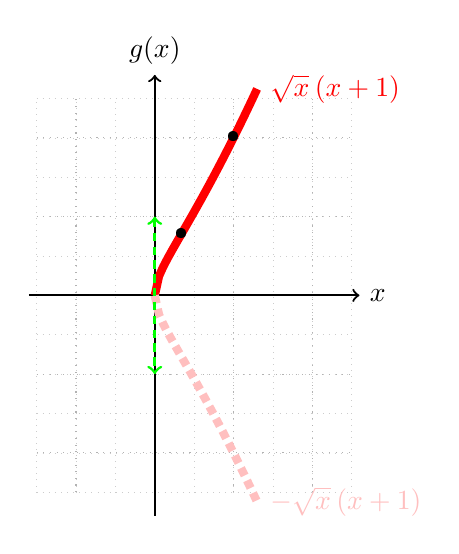
\begin{tikzpicture}[domain=0:1.3]
				\draw[dotted, very thin, gray!40, step=0.5] (-1.5,-2.5) grid (2.5,2.5) ;
				\draw[dotted, gray!60] (-1.5,-2.5) grid (2.5,2.5) ;
				\draw[->,thick] (-1.6,0) -- (2.6,0) node[right] {$x$};
				\draw[->,thick] (0,-2.8) -- (0,2.8) node[above] {$g(x)$};
				\draw[line width = 3pt,color=red] plot(\x,{sqrt(\x)*(1+\x)}) node [right] {$ \sqrt{x} \hskip 2pt (x+1)$};
				\draw[line width = 3pt,color=pink,densely dashed] plot(\x,{-sqrt(\x)*(1+\x)}) node [right] {$ -\sqrt{x} \hskip 2pt (x+1)$};
				\draw[<-> , line width = 1pt,color=green,densely dashed] (0,1)--(0,-1) ;
				\node at (0.333,0.77) {\textbullet};
				\node at (1,2) {\textbullet};
			\end{tikzpicture}
		\end{minipage}
		
		
		
	}
	\item  \question{ Montrer que 	le point $(-1,0)$ est un point isol\'e de la partie ${\cal C}=\{(x,y); f(x,y)=0\}$
	du plan, c'est-\`a-dire, le point $(-1,0)$ appartient \`a cette partie	et il existe un nombre r\'eel 
	$\varepsilon >0$ tel que 	$D_{\varepsilon} \cap {\cal C} =\{(-1,0)\}$ o\`u $D_{\varepsilon}$ est le disque ouvert centr\'e en $(-1,0)$ et de rayon $\varepsilon$. }
	\reponse{Dans la boule ouverte 	$\{(x,y,z);(x+1)^2+y^2+x^2 <1\} \subseteq \R^3$, on est notamment dans le demi espace $\{x<0\}$. Or si $x<0$ et $f(x,y)=0$ alors nécessairement $y^2 = x(x+1)^2 \geq 0$ ce qui ne laisse d'autre choix que d'avoir $(x+1)^2 =0$. 
		
		Par conséquent, le graphe
		$z=f(x,y)$ de la fonction $f$ ne rencontre le plan des $x$ et $y$ qu'au point
		$(-1,0)$. Par cons\'equent, l'intersection 
		$D \cap \cal C$ du disque
		\[
		D=\{(x,y); (x+1)^2+y^2<1\}
		\]
		avec $\cal C$ ne consiste qu'au point $(-1,0)$.}
%	\item \question{ \'Enoncer le th\'eor\`eme des fonctions implicites. }
%	\item  Montrer que, quel que soit le point 
%	$(x_0,y_0)$ de ${\cal C}$ distinct de $(-1,0)$,
%	au moins une des deux alternatives (i) ou (ii) ci-dessous est v\'erifi\'ee:
%	\begin{enumerate}
%		\item[(i)]
%		Il existe une fonction  $h$ de classe $C^1$ de la variable $x$ 
%		d\'efinie dans un intervalle ouvert 
%		appropri\'e telle que $h(x_0)=y_0$ et telle que,
%		pour qu'au voisinage de $(x_0,y_0)$
%		les coordonn\'ees $x$ et $y$ du point $(x,y)$
%		satisfassent \`a l'\'equation
%		$f(x,y)=0$ il faut et il suffit que
%		$y=h(x)$.
%		\item[(ii)]
%		Il existe une fonction  $k$ de classe $C^1$ de la variable $y$ 
%		d\'efinie dans un intervalle ouvert 
%		appropri\'e telle que $h(y_0)=x_0$ et telle que,
%		pour qu'au voisinage de $(x_0,y_0)$
%		les coordonn\'ees $x$ et $y$ du point $(x,y)$
%		satisfassent \`a l'\'equation
%		$f(x,y)=0$ il faut et il suffit que
%		$x=k(y)$.
%		\rep{Quel que soit le point 
%			$(x_0,y_0)$ de ${\cal C}$
%			distinct de  $(-1,0)$,
%			d'apr\`es (1.),
%			\[
%			\left(\frac{\partial f}{\partial x}(x_0,y_0),\frac{\partial f}{\partial y}(x_0,y_0) \right) 
%			\ne (0,0).
%			\] 
%			L'assertion est donc une cons\'equence imm\'ediate du th\'eor\`eme des 
%			fonctions implicites. }
%	\end{enumerate}
	
\end{enumerate}}
